%!TEX root = ../bachelor.tex
\chapter{Fazit und Ausblick}
Parallelisierung?

delaunay? lohnt sich eigentlich nicht, weil reverse sehr gute ergebnisse

deformable templates als alternative zu ransac für ellipsen?  probleme mit lokalen minima



deformable templates

evtl noch am ende delaunay

iteratives verfahren zum minimieren des reprojection fehlers ausprobieren



\begin{figure}[!htb]
	\centering
	\begin{subfigure}{.9\textwidth}
		\centering
		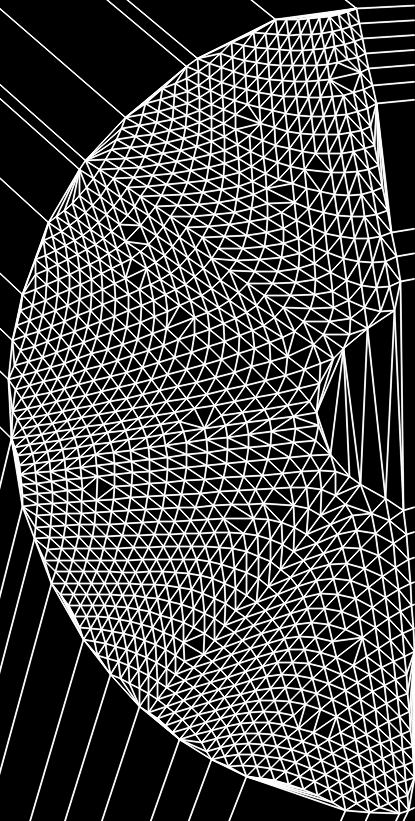
\includegraphics[angle=-90, width=.8\textwidth]{images/delaunay1.png}
		\caption{del1}
	\end{subfigure}
	\begin{subfigure}{.9\textwidth}
		\centering
		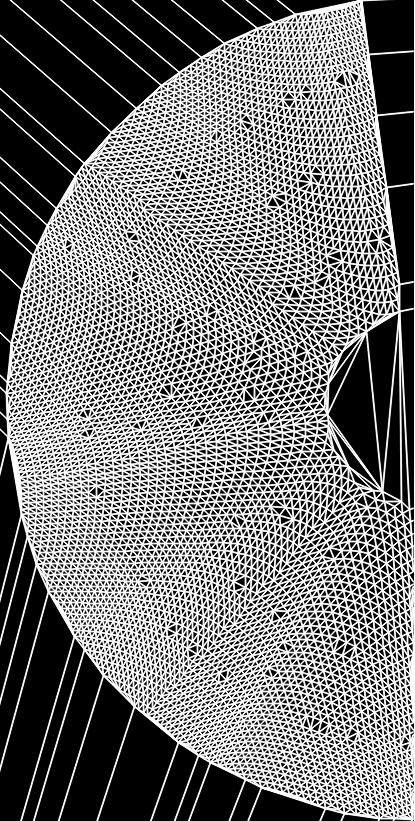
\includegraphics[angle=-90, width=.8\textwidth]{images/delaunay2.png}
		\caption{del2}
	\end{subfigure}
	\label{fig:delaunay}
	\caption{Delaunay}
\end{figure}